\chapter{METODOLOGÍA DE LA INVESTIGACIÓN}

En este capítulo se describe la metodología empleada en el desarrollo de la investigación. Se detallan el diseño de investigación, tipo y enfoque, así como el alcance del estudio. Además, se presentan las estrategias para la recolección y análisis de datos, orientadas a evaluar la efectividad de una aplicación móvil basada en Inteligencia Artificial generativa para el soporte integral a pacientes con cáncer de mama.

\section{Diseño, tipo y enfoque de la investigación}

\subsection{Diseño}

El diseño de la investigación es de tipo experimental, dado que se busca analizar la interacción de los pacientes con la aplicación móvil y evaluar los cambios en su estado de salud y bienestar. Este diseño permite observar los efectos directos del uso de la tecnología en un entorno controlado, mediante la implementación de pruebas piloto en condiciones reales. El nivel de la investigación es explicativo, ya que tiene como objetivo establecer relaciones causales entre el uso de la aplicación y la mejora en el soporte integral ofrecido a los pacientes. Se busca determinar si el empleo de IA generativa en la aplicación contribuye significativamente al monitoreo, control y soporte emociona.

\subsection{Enfoque}
El enfoque adoptado es cuantitativo, lo que permite medir objetivamente variables como la adherencia al tratamiento, la precisión de las predicciones generadas por la IA y la satisfacción del usuario. Este enfoque se sustenta en la recolección de datos numéricos para su posterior análisis estadístico

\subsection{Alcance de la investigación}
El alcance de este estudio se centra en identificar y explicar la relación entre el uso de la aplicación móvil y la mejora en el soporte integral a pacientes con cáncer de mama. La investigación tiene un propósito explicativo, ya que busca profundizar en cómo la tecnología puede impactar positivamente en la experiencia de los pacientes, tanto en aspectos físicos como emocionales

\section{Población y muestra}

\subsection{Población}
La población objetivo de este estudio está conformada por mujeres diagnosticadas con cáncer de mama en etapa temprana o avanzada, que se encuentren en tratamiento en hospitales públicos, clínicas privadas, o que, de manera independiente, deseen participar en el estudio. Esto abarca pacientes de diversas condiciones socioeconómicas y niveles de acceso a servicios de salud en Lima, Perú.
\subsection{Muestra}

El muestreo será no probabilístico por conveniencia, enfocado en mujeres que cumplan con los criterios de inclusión y que voluntariamente acepten participar. Esto permitirá evaluar la efectividad de la aplicación en diversos contextos y niveles de acceso a la atención médica. Donde la muestra estará compuesta entre 5 a 15 pacientes con cáncer de mama por la complejidad de la enfermedad, quienes serán seleccionadas a través de las siguientes vías:

\begin{itemize}
\item \textbf{Hospitales públicos:} \\
Pacientes en tratamiento en instituciones de salud pública, con el debido permiso y coordinación con los centros de salud.
\item \textbf{Clínicas privadas:} \\
Pacientes en tratamiento en centros de atención privada, previa autorización de las clínicas.
\item \textbf{Clínicas privadas:} \\
Pacientes en tratamiento en centros de atención privada, previa autorización de las clínicas.
\item \textbf{Clínicas privadas:} \\
Pacientes en tratamiento en centros de atención privada, previa autorización de las clínicas.
\item \textbf{Anuncios públicos:} \\
Se difundirá un llamado abierto para que cualquier mujer diagnosticada con cáncer de mama, interesada en participar, pueda inscribirse voluntariamente en el estudio.
\end{itemize}

\textbf{Unidad de análisis:}
La unidad de análisis será cada paciente, enfocándose en medir el impacto de la aplicación móvil en aspectos como el monitoreo de signos vitales, la adherencia al tratamiento y el soporte emocional proporcionado.

\section{Operacionalización de Variables}
Matriz de variables principales

\begin{table}[H]
\centering
\renewcommand{\arraystretch}{1.8} % Espaciado entre filas
\setlength{\tabcolsep}{5pt} % Espaciado horizontal en celdas
\begin{tabular}{|p{5cm}|p{4cm}|p{6cm}|}
\hline
\textbf{VARIABLE Y DEFINICIÓN} & \textbf{INDICADOR} & \textbf{FÓRMULA DE INDICADOR} \\ \hline

\parbox[t]{5cm}{\textbf{Adherencia al tratamiento} \\ Cumplimiento de las pautas médicas por parte de los pacientes con cáncer de mama.} 
& Porcentaje de seguimiento al tratamiento cumplido & 
$\frac{\text{N°Tratamiento completadas*100}}{\text{N°de tratamientos preescritos}}$ \\ \hline

\parbox[t]{5cm}{\textbf{Soporte emocional} \\ Capacidad de la aplicación para mejorar el bienestar emocional de las pacientes.} 
& Porcentaje de seguimiento al tratamiento cumplido & Encuestas de satisfacción en escala Likert \\ \hline

\parbox[t]{5cm}{\textbf{Monitoreo de signos vitales} \\ Supervisión constante de parámetros como la frecuencia cardíaca y temperatura.} 
& Precisión en la detección de anomalías & $\frac{TP+TN}{TP + FP}$ \\ \hline

\parbox[t]{5cm}{\textbf{Modelo de inteligencia artificial} \\ Evaluación de la eficacia del modelo implementado en la aplicación móvil.} 
& Accuracy & $\frac{TP + TN}{TP + FP + FN + TN}$ \\ \cline{2-3}
& Precision & $\frac{TP}{TP + FP}$ \\ \cline{2-3}
& Recall & $\frac{TP}{TP + FN}$ \\ \cline{2-3}
& F1 & $\frac{2 \cdot \text{Precision} \cdot \text{Recall}}{\text{Precision} + \text{Recall}}$ \\ \cline{2-3}
& ROC AUC & $P(\text{score}(x^+) > \text{score}(x^-))$ \\ \hline

\end{tabular}
\caption{Matriz de variables principales para el soporte intregral de pacientes con cáncer de mama.}
\label{table:variables}
\end{table}

\vspace{1.5 cm}


\textbf{Donde:}
\begin{itemize}
    \item TP = True Positives
    \item FP = False Positives
    \item FN = False Negatives
    \item TN = True Negatives
\end{itemize} 


\section{Técnicas de recolección de datos}


La recolección de datos se realizará mediante tres principales fuentes, con el fin de obtener información cuantitativa y cualitativa que permita evaluar la efectividad de la aplicación móvil en el soporte integral a pacientes con cáncer de mama:

\begin{enumerate}
    \item \textbf{Encuestas}\\
    Se aplicarán encuestas estructuradas a las pacientes participantes para medir su percepción y satisfacción respecto al uso de la aplicación móvil. Las encuestas incluirán preguntas sobre:
    \begin{itemize}
        \item \textbf{Satisfacción emocional:} Nivel de soporte emocional proporcionado por la aplicación.
        \item \textbf{Usabilidad:} Facilidad de uso y comprensión de las funciones de la aplicación.
        \item \textbf{Percepción de mejora:} Opiniones sobre la adherencia al tratamiento y la utilidad del monitoreo.
    \end{itemize}
    \textbf{Formato:} Escala Likert de 1 a 5, donde 1 representa ``muy insatisfecha'' y 5 ``muy satisfecha''.
    
    \item \textbf{Registros médicos}\\
    Se recopilarán registros médicos de las participantes que permitan verificar su adherencia al tratamiento. Estos incluirán:
    \begin{itemize}
        \item Número de citas médicas programadas y asistidas.
        \item Cumplimiento de sesiones de quimioterapia o radioterapia.
        \item Resultados de análisis médicos relacionados con el seguimiento del cáncer de mama.
    \end{itemize}
    Este tipo de información será contrastado con los datos proporcionados por la aplicación para validar su precisión.
    
    \item \textbf{Datos generados por la aplicación móvil}\\
    La aplicación almacenará y analizará automáticamente datos clave sobre el uso y el estado de las pacientes, tales como:
    \begin{itemize}
        \item \textbf{Monitoreo de signos vitales:} Frecuencia cardíaca, temperatura corporal y otros parámetros vitales.
        \item \textbf{Alertas y notificaciones:} Registro de alertas enviadas y las acciones tomadas por las pacientes.
        \item \textbf{Interacción con el soporte emocional:} Frecuencia y tipo de respuestas proporcionadas por el sistema de IA generativa.
    \end{itemize}
    Todos estos datos son exportados en formatos estructurados (por ejemplo, \texttt{.csv} o bases de datos SQL) para su posterior análisis estadístico.
\end{enumerate}

\section{Técnicas para el procesamiento y análisis de la información}
\subsection{Metodología de la solución}
\begin{figure}[ht]
	\centering
	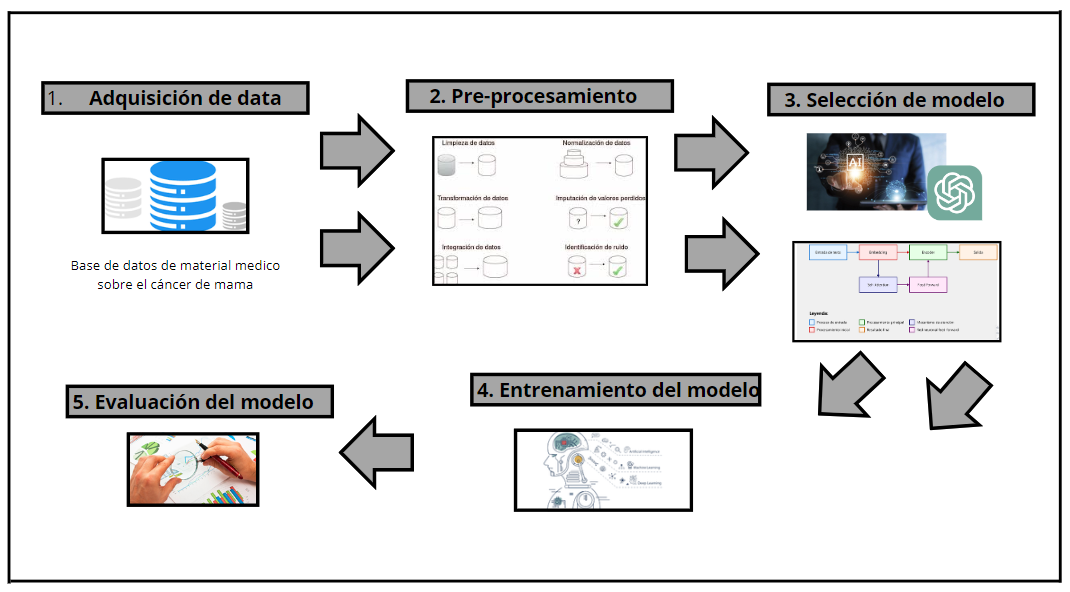
\includegraphics[width=\textwidth]{3/figures/MIsolucion.png}
	\caption{Metodología de la investigación}
	\label{14:fig}
\end{figure}
\begin{figure}[ht]
	\centering
	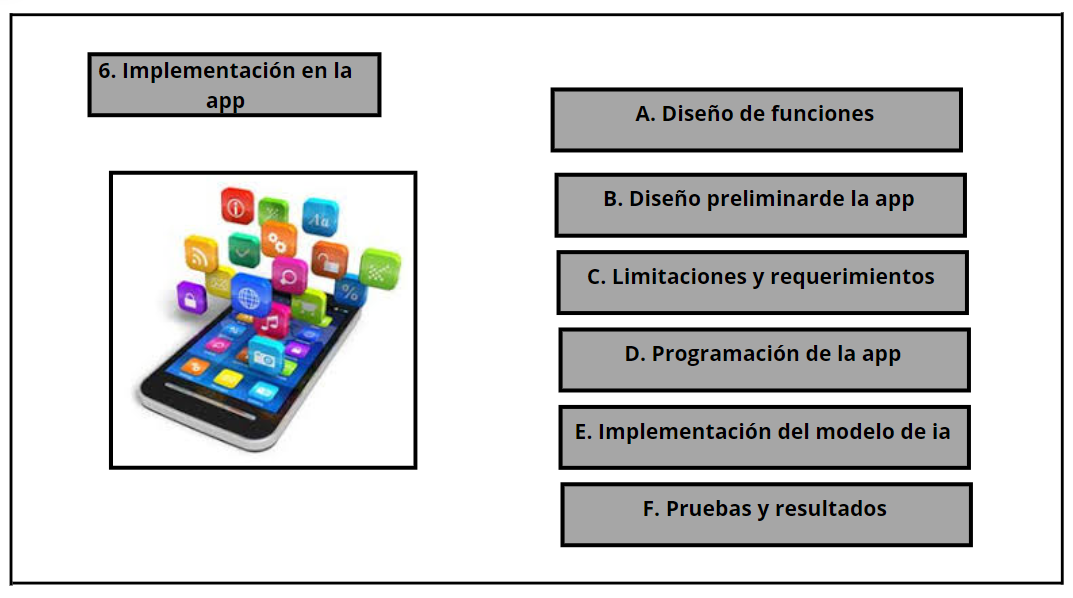
\includegraphics[width=\textwidth]{3/figures/MI2.png}
	\caption{Metodología de la investigación}
	\label{14:fig}
\end{figure}

\subsubsection{Adquisición de Datos}
La calidad de los datos es fundamental para entrenar un modelo de IA generativa efectivo. Este paso debe garantizar datos ricos, diversos y representativos del dominio médico y emocional.

\textbf{Fuentes de datos específicas:}
\begin{itemize}
    \item \textit{Bases de datos textuales médicas:} PubMed, MIMIC-III (datos clínicos anonimizados), OncoKB, guías clínicas internacionales como NCCN Guidelines y ESMO Guidelines.
    \item \textit{Transcripciones de interacciones médico-paciente:} Conversaciones reales o simuladas representativas de preguntas y respuestas comunes.
    \item \textit{Datos emocionales o psicológicos:} Encuestas sobre ansiedad y estrés en pacientes oncológicos, datos de plataformas de telemedicina y análisis de textos en foros.
\end{itemize}

\textbf{Proceso de recopilación:}
\begin{itemize}
    \item Colaboraciones con hospitales o clínicas para obtener datos anonimizados.
    \item Uso de bases públicas disponibles.
    \item \textit{Web scraping} en páginas confiables con permisos legales.
\end{itemize}

\textbf{Normativas éticas:}
\begin{itemize}
    \item Cumplir con estándares como GDPR o HIPAA para garantizar privacidad.
    \item Revisiones éticas continuas durante todo el proceso.
\end{itemize}

\subsection{Preprocesamiento de Datos}
El preprocesamiento asegura que los datos estén organizados y listos para ser utilizados por el modelo.

\textbf{Pasos principales:}
\begin{itemize}
    \item \textit{Limpieza del texto:} Eliminación de información irrelevante, corrección de errores tipográficos, y normalización de abreviaturas médicas.
    \item \textit{Tokenización:} Dividir los textos en palabras, subpalabras o frases según el enfoque del modelo.
    \item \textit{Etiquetado:} Clasificar información en categorías como diagnóstico, tratamiento, emociones y preguntas frecuentes.
    \item \textit{Normalización:} Convertir textos a minúsculas, eliminar caracteres especiales y estandarizar unidades médicas.
\end{itemize}

\textbf{Enriquecimiento de datos:}
\begin{itemize}
    \item Realizar \textit{data augmentation} textual para diversificar el dataset.
\end{itemize}


\subsection{Selección del Modelo}
Dado que el objetivo es implementar un modelo generativo eficiente, los Transformers son la elección más adecuada.

\textbf{Modelos a considerar:}
\begin{itemize}
    \item \textit{GPT (Generative Pre-trained Transformer):} Ideal para generar respuestas empáticas y médicamente correctas.
    \item \textit{T5 (Text-to-Text Transfer Transformer):} Versátil para tareas de entrada y salida de texto.
    \item \textit{BERT:} Orientado a la comprensión textual, útil como complemento para análisis de estados emocionales.
    \item \textit{Vision Transformers (ViT):} Opcional si se incluyen imágenes médicas.
\end{itemize}


\subsubsection{Motivación}
\begin{itemize}
    \item Los Transformers tienen capacidades avanzadas para manejar texto contextual y tareas personalizadas.
\end{itemize}

\subsection{Entrenamiento del Modelo}
El entrenamiento es la etapa más crítica y se divide en varias subfases.

\textbf{Preparación del entrenamiento:}
\begin{itemize}
    \item \textit{División del dataset:}
    \begin{itemize}
        \item \textbf{70-80\% entrenamiento:} Ajuste de pesos del modelo.
        \item \textbf{10-15\% validación:} Optimización de hiperparámetros y evaluación durante el proceso.
        \item \textbf{10-15\% pruebas:} Evaluación de precisión final.
    \end{itemize}
    \item \textit{Hiperparámetros clave:}
    \begin{itemize}
        \item Tamaño del \textit{batch:} 16-64 (dependiendo de la GPU).
        \item Tasa de aprendizaje: 1e-4 o 1e-5 para modelos preentrenados.
        \item Número de \textit{epochs:} 20-50 según el tamaño del dataset.
    \end{itemize}
\end{itemize}

\textbf{Técnicas de entrenamiento:}
\begin{itemize}
    \item \textit{Fine-tuning:} Adaptación de modelos preentrenados al dominio específico.
    \item \textit{Entrenamiento desde cero:} Útil si se requieren características únicas no presentes en modelos existentes.
    \item \textit{Regularización:} Uso de técnicas como Dropout para evitar sobreajuste.
\end{itemize}

\subsection{Evaluación del Modelo}
La evaluación asegura que el modelo funcione correctamente y sea útil para los pacientes y médicos.

\textbf{Métricas de desempeño:}
\begin{itemize}
    \item \textit{Perplejidad:} Evalúa la capacidad del modelo para predecir palabras.
    \item \textit{BLEU/ROUGE:} Miden la similitud entre el texto generado y de referencia.
    \item \textit{Validación con expertos:} Médicos revisan las respuestas generadas.
    \item \textit{Pruebas A/B:} Comparación con métodos tradicionales.
\end{itemize}

\section{Cronograma de actividades y presupuesto (Hasta la fecha actual}
\subsection{Cronograma de actividades}
\begin{figure}[ht]
	\centering
	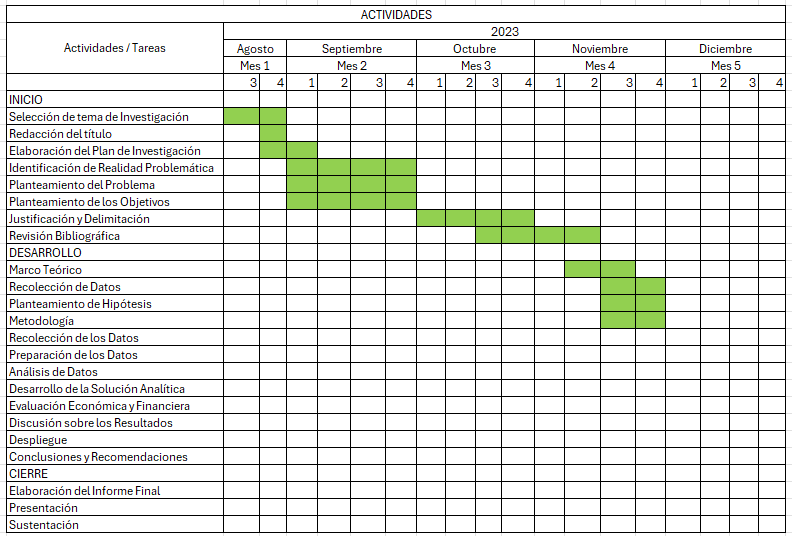
\includegraphics[width=\textwidth]{3/figures/Cronograma de actividades hasta la fecha.png}
	\caption{Cronograma de actividades}
	\label{15:fig}
\end{figure}

\subsection{Presupuesto}
\begin{figure}[ht]
	\centering
	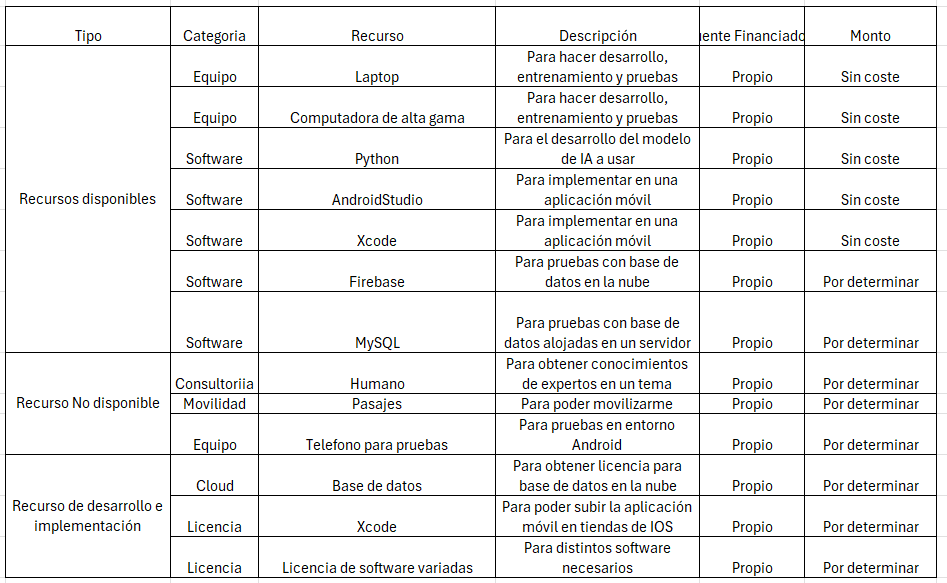
\includegraphics[width=\textwidth]{3/figures/Recursos.png}
	\caption{Recursos necesarios}
	\label{16:fig}
\end{figure}
